中国移动的OneNET平台专门为物联网应用开发,我们可以使用ESP32连接到MQTT服务器,之后再构建手机APP来获取数据,真正实现信息互联。

\subsubsection{构建OneNET平台鉴权token}
OneNET平台:\href{https://open.iot.10086.cn/}{\underline{https://open.iot.10086.cn/}}
我使用的是OneJSON数据结构,MQTT协议上传。

将一些基础信息置于此地,后续需要时在这里查看:(鉴权Token在后节获得)
\begin{itemize}
    \item 设备密钥:VzZrREE0T2hYeDZ0dDFQSUZZWWRIZ29yMGxrRUdGY2g=
    \item 设备名称:DHT22
    \item 产品ID:W9TI0JaXlu
    \item 产品Access:8fnx/QsBBf/BUeWpU68j4bG7iwNVm315g+vzc8c
    \item 鉴权Token:version=2018-10-31\&res=products\%2FW9TI0JaXlu\%2Fdevices\%2FDHT22\&et=1759306118\&method=md5
    \item \&sign=JRsZv0peZQOTmr7Eg8lGJg\%3D\%3D
\end{itemize}

在PlatformIO中使用PubSubClient库,可以用于在Arduino框架下实现MQTT通信。下面,通过OneNET平台的官方文档找到了接口:\href{https://open.iot.10086.cn/doc/v5/fuse/detail/919}{\underline{https://open.iot.10086.cn/doc/v5/fuse/detail/919}}

\begin{figure} [H]
    \centering
    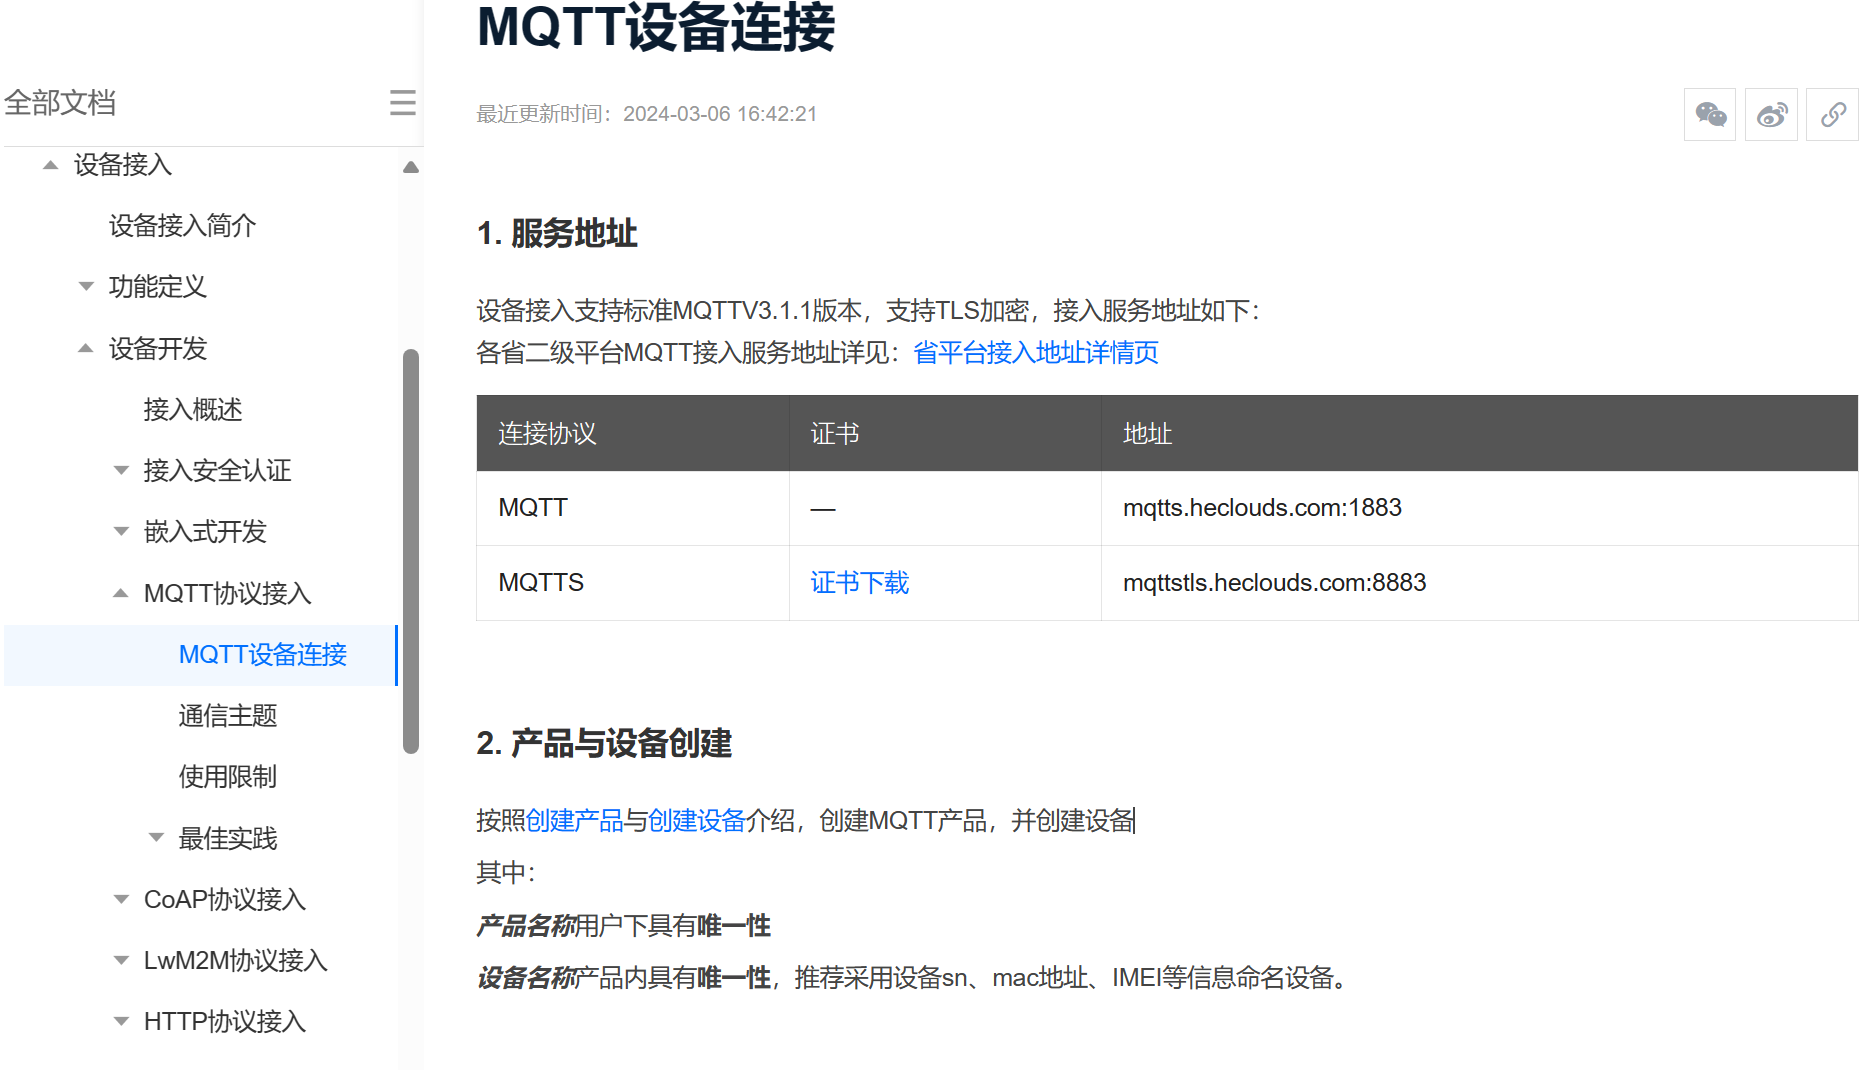
\includegraphics[width=0.7\textwidth]{img/MQTTInit.png}
    \caption{OneNET平台接口}
\end{figure}

按照文档:产品、设备创建时,平台为每类产品、每个设备均分配了唯一的 key,设备登录时需要使用通过key计算出的访问token 来进行访问安全认证。
官方提供了token计算工具,按照res使用场景根据步骤获得token。

\begin{figure} [H]
    \centering
    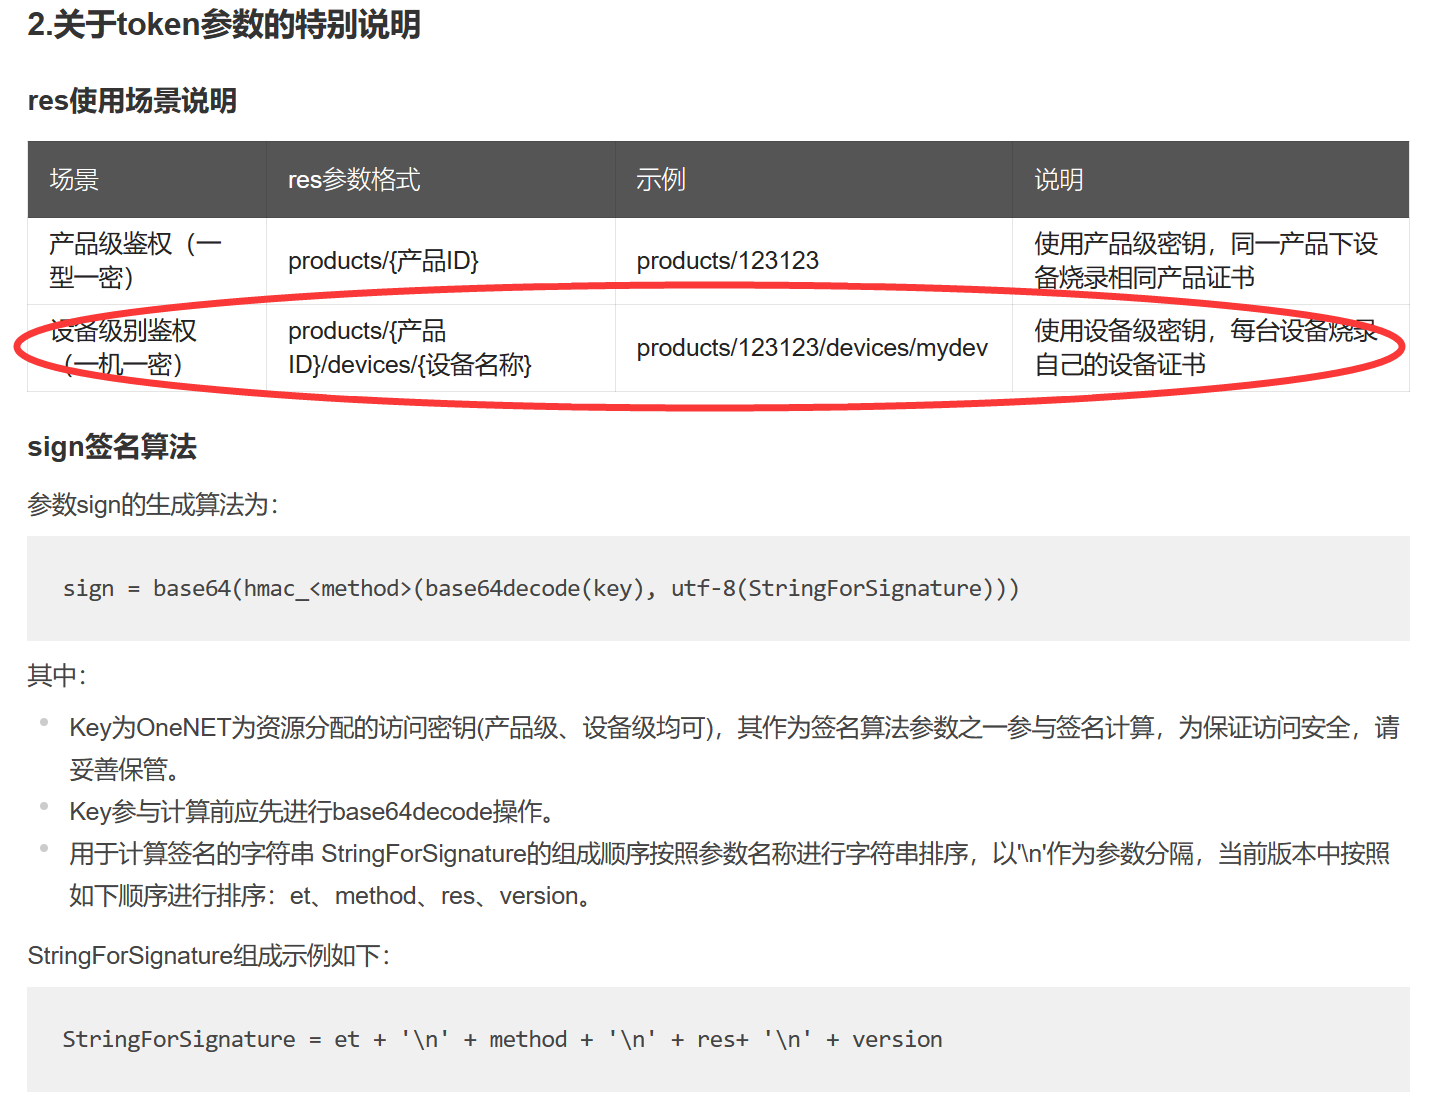
\includegraphics[width=0.5\textwidth]{img/MQTT_Auth.png}
    \caption{OneNET平台token计算}
\end{figure}

在调用讯飞API时我使用的就是Sha-256算法,根据官方文档,支持md5、Sha-1、Sha-256,故我使用Sha-256作为尝试。
注意,官方文档中提到:

\begin{figure} [H]
    \centering
    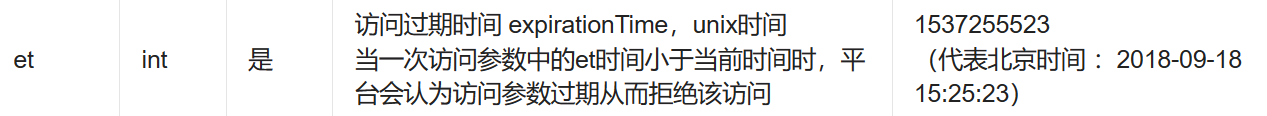
\includegraphics[width=0.5\textwidth]{img/Noteet.png}
    \caption{et代表过期时间}
\end{figure}

故使用Unix时间戳转换工具,将到期时间设置为2025年10月1日。

Unix时间戳转换网址为:\href{https://www.jyshare.com/front-end/852/}{\underline{https://www.jyshare.com/front-end/852/}}
,转换得到1759306118。

\begin{figure} [H]
    \centering
    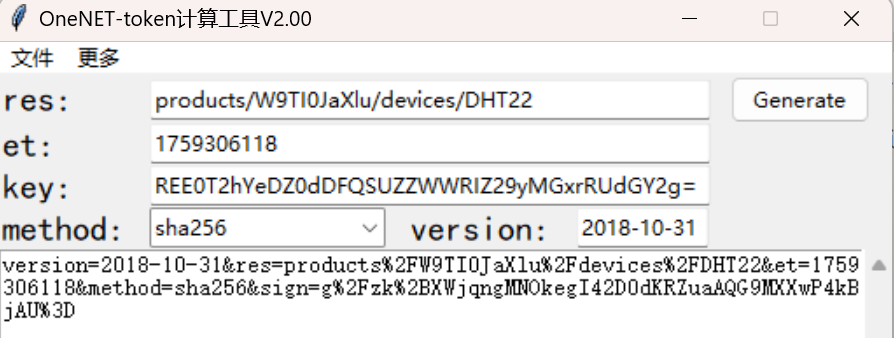
\includegraphics[width=0.5\textwidth]{img/MQTT_sha256.png}
    \caption{计算工具}
    \label{fig:MQTT_sha256}
\end{figure}

\subsubsection{连接到MQTT服务器}

连接到MQTT服务器的关键部分代码如下所示:

\begin{lstlisting}[language=C++, title=MQTT Connect]
    WiFiClient espClient;
    PubSubClient client(espClient);

    void connectOneNet() {
        client.setServer(MQTT_Server.c_str(), MQTT_Port);
        bool isConnected = client.connect(MQTT_Device_ID.c_str(), MQTT_Product_ID.c_str(), MQTT_Token.c_str());
    }

    void loop() {
        client.loop();
    }
\end{lstlisting}

\begin{figure} [H]
    \centering
    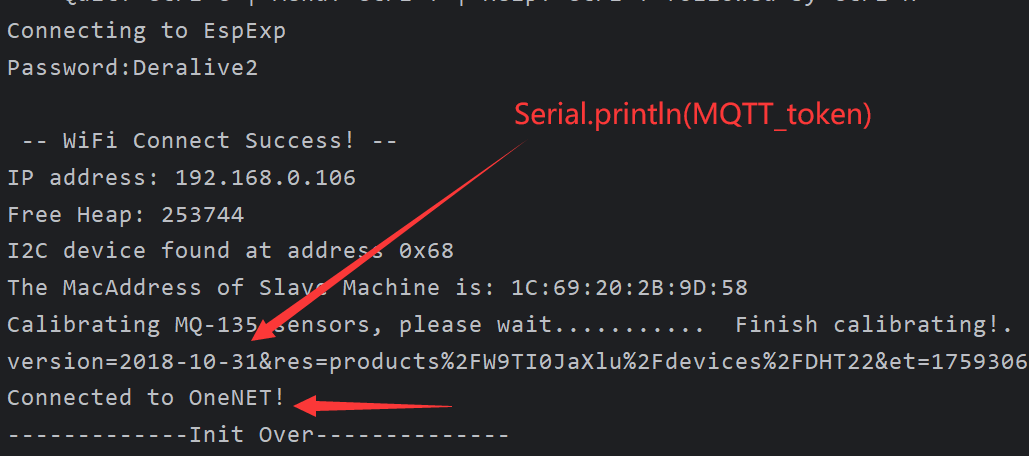
\includegraphics[width=0.5\textwidth]{img/MQTTConnected.png}
    \caption{MQTT服务器连接成功}
\end{figure}

\subsubsection{与MQTT服务器进行数据交互}

连接到服务器后,数据的上传和下载自然成为接下来要攻克的主题。这两部分分别从属于“发布”与“订阅”的操作权限。

\begin{figure} [H]
    \centering
    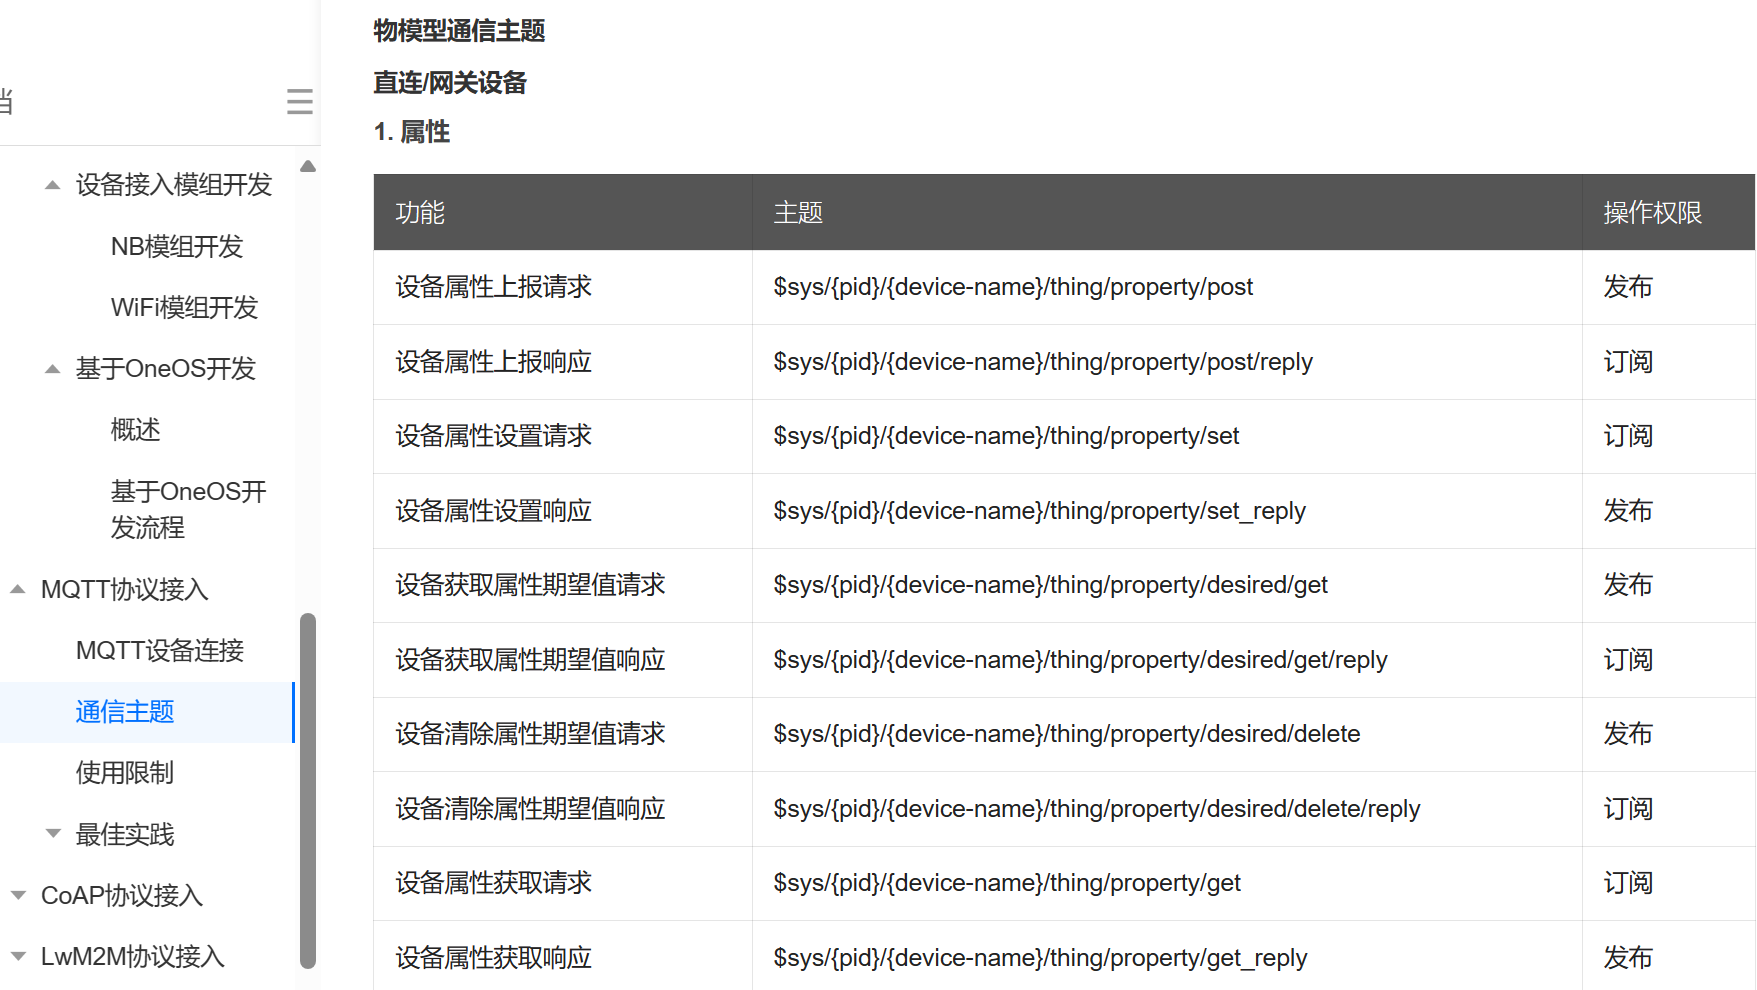
\includegraphics[width=0.6\textwidth]{img/MQTTSubscribe.png}
    \caption{MQTT发布}
\end{figure}

往下翻,需要向服务器传输JSON格式的字符串,如下图所示:

\begin{figure} [H]
    \centering
    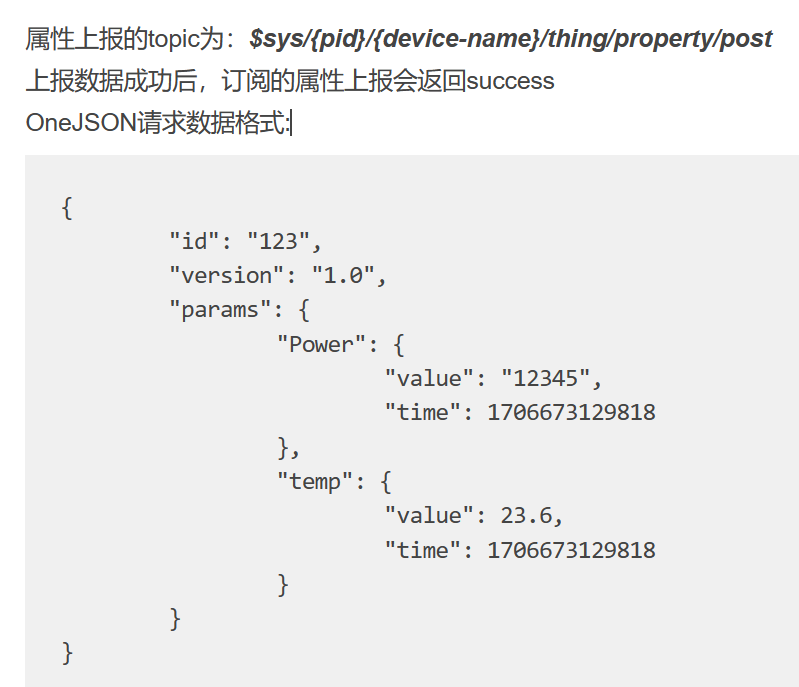
\includegraphics[width=0.3\textwidth]{img/MQTTSendJson.png}
    \caption{MQTT Send Data With JSON Format}
\end{figure}

关键函数如下所示,注意要看物模型通信主题中哪一个是订阅,哪一个是发布。
使用对应的函数\texttt{client.subscribe() 或 client.publish()},同时,设置回调函数mqttCallback(),用于处理服务器返回的数据。
回调函数解析服务器返回的数据,若为 200 则代表数据解析成功。

此处的每一个函数返回的都是boolean类型(可以通过点入函数声明的部分,即在PubSubClient.cpp内查阅),使用返回值来做对应的串口输出,用于提示我是否完成了此次请求。
关键代码如下所示:

\begin{lstlisting} [language=C++, title=MQTT Publish and Subscribe] 
    void connectOneNet() {
        client.setServer(MQTT_Server.c_str(), MQTT_Port);
        client.setCallback(mqttCallback); // 回调函数解析服务器返回的数据,若为 200 则代表数据解析成功

        bool isConnected = client.connect(MQTT_Device_ID.c_str(), MQTT_Product_ID.c_str(), MQTT_Token.c_str());
        bool isSubscribeProperty = client.subscribe(ONENET_TOPIC_PROP_SET); //订阅设备属性设置请求
        bool isSubscribeUpdata = client.subscribe(ONENET_TOPIC_PROP_POST_REPLY); //订阅设备属性上报响应

        if (isConnected) {
            Serial.println(F("Connected to OneNET!"));
        } else {
            Serial.println(F("Failed to connect OneNeT!"));
        }
        // 更多 if,结构一致,为节省篇幅,省略。

        ticker.attach(3,OneNET_Prop_Post); // 使用 Ticker 对象,每隔 3 秒发送一次设备属性上报。
    }
    
    void OneNET_Prop_Post() {
        if (client.connected()) {
            char parameters[256];
            char jsonBuff[256];

            // 构建用来传输至 MQTT 服务器的 JSON 数据
            sprintf(parameters, "{\"temperature\":{\"value\":%.2f},\"humidity\":{\"value\":%.2f}}",dht22Data.temperature,dht22Data.humidity);
            sprintf(jsonBuff,ONENET_TOPIC_PROP_FORMAT,postMessageID++,parameters);
            // 按照文档,#define ONENET_TOPIC_PROP_FORMAT "{\"id\":\"%u\",\"version\":\"1.0\",\"params\":%s}"

            bool isUpData = client.publish(ONENET_TOPIC_PROP_POST, jsonBuff);
        }
    }
    
    void mqttCallback(char* topic, byte* payload, unsigned int length) {
        // 将接收到的消息转换为字符串
        char message[length + 1];
        strncpy(message, (char*)payload, length);
        message[length] = '\0';
    
        // 打印主题和消息内容
        Serial.print("Received message from topic: ");
        Serial.println(topic);
        Serial.print("Message: ");
        Serial.println(message);
    }
\end{lstlisting}

将信息发送至MQTT服务器及服务器接收得到的结果如图所示:

\begin{figure} [H]  
    \centering
    \begin{subfigure}[t]{0.8\textwidth}
        \centering
        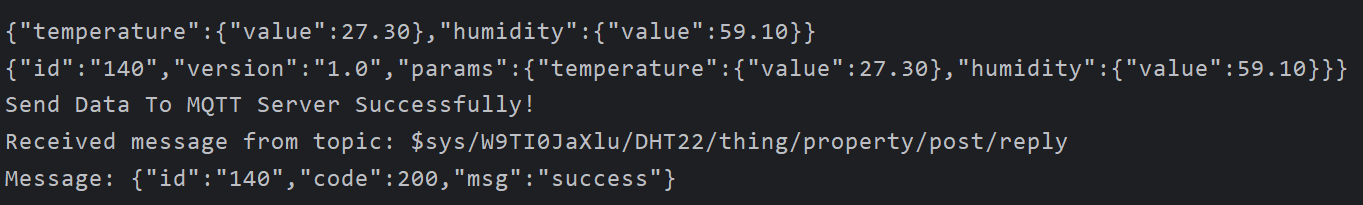
\includegraphics[width=\textwidth]{img/MQTTSendSuccess.png}  
        \caption{将信息发送至MQTT服务器}
        \label{fig:SendToMQTT}
    \end{subfigure}
    
    \vspace{1em}
    
    \begin{subfigure}[t]{0.6\textwidth}
        \centering
        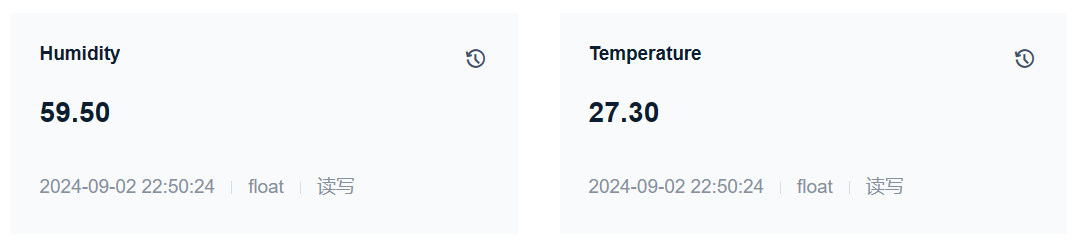
\includegraphics[width=\textwidth]{img/MQTTGetData.png}  
        \caption{OneNET服务器接收到数据}
        \label{fig:OneNETGet}
    \end{subfigure}
    
    \caption{MQTT 发送与接收}
\end{figure}

接下来要做的事情和上面的重复,把其他传感器和想要的数据传输到上面即可。

\begin{figure} [H]
    \centering
    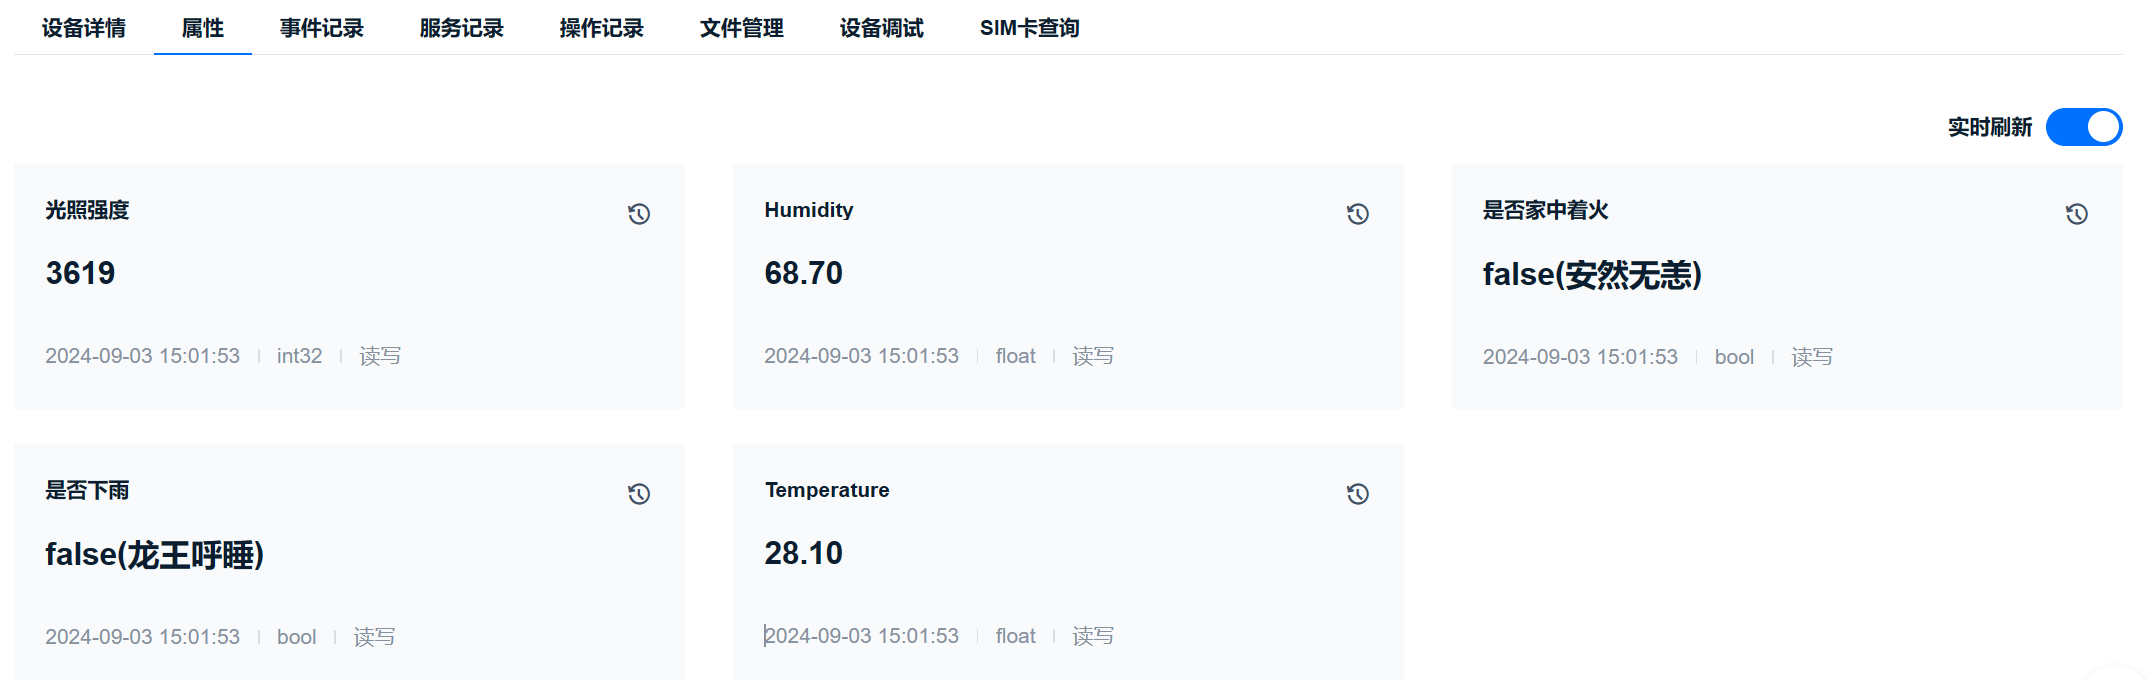
\includegraphics[width=0.5\textwidth]{img/MQTT_Data.png}
    \caption{MQTT服务器接收到的数据}
\end{figure}